\documentclass[12pt]{article}
\usepackage{amsmath}
\usepackage{amssymb}
\usepackage{graphicx}
\usepackage[margin=0.5in]{geometry}
\newcommand{\del}{\nabla}
\begin{document}

\title{Kronecker Graphs for Modelling Linguistic Data}
\author{Howon Lee (howonlee at stanford.edu)}
\maketitle

\section{Abstract}

%%% abstract would be nice

\section{Introduction, Literature Review, Problem}

An important statistical regularity in language is Zipf's law. It says that given some corpus of natural language, the frequency of any word is inversely proportional to its rank on the frequency table: the frequency is distributed according to a power law, in other words, meaning a probability distribution of the form:

$$p(x) Cx^{-\alpha} $$

where $C$ is a normalizing constant.

However remarkable it may be, however, Zipf's law is not yet a statement about the structure of language. This is because it holds for corpuses as bags of words which have frequencies, not as linguistic entities which have structure. \cite{smallworldlang}

One important language model ubiquitous in NLP which incorporates some aspect of linguistic structure, notably without specification, is the n-gram, which takes the semi-Markov assumption that the only context needed to reproduce a word is the past $n$ words. This is of interest, because it turns out that thinking of a corpus as a graph of words and the order-one and order-two relations between words, as bigram and trigram models do, reveals many small-world properties in the structuring of words in corpuses.

We want to deal with the problem of using and adapting already existing algorithms for creating small world nets by creating a parsimonious model of language with Kronecker graphs that respects these network properties of words as they currently exist. We used that language model for a part-of-speech tagging task, and for a language generation task, and show that an aspect of the structure of the generated graph can be used as a feature for the part-of-speech tagging task.

Language is only one of many places where power laws are found, and a power law may be explained by one of a multiplictiy of possible causes. MEJ Newman gives a review \cite{mejpowerlaw}. Among the properties of power laws is that, depending on the parameter, the first and second moments can be infinite. That is, the average number of inhabitants of a city is on the order of $10^3$. If the populations of cities were distributed according to the Gaussian, Tokyo would be stupendously unlikely, basically impossible.

A particular point of interest is the introduction to a possible information-theoretic origin of Zipf's law. MEJ Newman reviews a possible origin of power law phenomena in language due to Miller\cite{gamiller}. Miller's argument goes like this: imagine a monkey typing on a typewriter, delimiting words with some probability and writing a random letter with some uniform probability. Then, this approximates an exponential distribution of frequency of a word $x$ with number of letters $y$. But the number of possible words goes up exponentially with $y$ also, making the distribution of frequencies a combination of exponentials, which is a power law.

This is a simplistic argument, but can be made less simplistic in talking about arbitrary information in bits instead of symbols in a normal alphabet. However, this theory is only compatible with a random typewriter of information with independence of the typing. However, the example of Shannon's entropy game, where one guesses the next word based upon the previous word in a communication, implies that some conditional structure exists in language, since humans can play Shannon's entropy game. \cite{shannon}
. 

A possible model of small world graphs is the stochastic Kronecker graph\cite{kronfit}, which is a sample from a distribution over graphs created by drawing a fractal over an adjacency matrix using the Kronecker product operation. The important thing about this model is that it tries to simultaneously fulfill the many observed properties of small world graphs, not just the heavy tail for indegree and outdegree, but also the heavy tail for scree plots, the densification power law, and small diameters, all at the same time.

The novel contribution of this paper is to note that the parameters for that distribution can be fitted with KronFit, a gradient descent algorithm which learns much bigger graphs much faster than previous attempts to fit graphs like the exponential random graph. This is because it uses MCMC to assign node labels and because it uses the sparsity of the small world graph to estimate the likelihood in time linear to the number of edges instead of quadratic to the number of nodes. The number of parameters is determined using a BIC metric.

There are also real interpretations of the Kronecker product process in the structure and creation of graphs. One intuition is that networks are hierarchically organized into communities, which grow recursively, creating miniature copies of themselves. Another interpretation is to say that each node is described by a sequence of categorical features, and the probability of two nodes linking depends on the product of individual attribute similarities, which allows modelling of homophily and heterophily at the same time.

One important point to take into mind is that one suggested usage for the Kronecker fitting algorithm is for compression of graphs. This is important, because whenever we hear "compression" we should smell "machine learning", because any system of compression can be used for prediction, by finding the symbol that compresses best given the history of the data \cite{mlcompression}.

Instead of talking about syntactic structure in sentences, it is possible investigate the statistical structure of these mere co-occurrences, and this was the method of Cancho and Sole. Why? Four reasons. It's easier to examine link structures automatically, as opposed to syntactic structures. They don't know what types of links there are in the structures of words, but just having the propinquity of words will capture almost every type. They are not interested in all the links, so looking at whole sentences will not be as productive. Long-distance syntactic links imply the existence of lower-distance syntactic links, but not vice versa.

Looking at the graph created in this way, they find small-world properties like high clustering coefficient, small diameter and power law degree distribution. They hypothesize that this leads to words that exist to speed up navigation in this small world, words like "and", "the", "of", "in", which do not contribute meaning but structure to grammar. They also hypothesize that the disfluency caused in agrammatism is caused by disruption to this small world.

If we take the central thesis of RF Cancho and RF Sole's work to be true, then word networks are small world networks. Therefore, they should be able to be fitted to parameters for a Kronecker distribution, which would compress the language graph to a very few parameters. It should be investigated whether these parameters, this model has any value as a language model.

The problems that this model should be used in is a part-of-speech tagger and in a generative model. The generative model should be used to generate text, and examined to see if it generates reasonable test. The language model should also be put into a POS tagger as a prior for the optimization target in a noisy channel model: there, the model would be of the distribution of the tags, which would require that the POS tags have a Zipf-like distribution of that sort. \cite{collins}

\subsection{Methods}
We used the annotated Brown corpus for the model, along with the tags that come with it on NLTK, so the Penn Treebank. The Brown corpus is a general corpus of English, in different genres such as news, religion, fiction, and government documents. There are 1161192 words in the corpus, in 57340 sentences, from a vocabulary of 56057 words, and 455267 unique bigrams. A train-test split was done of $\frac{2}{3}$ of the sentences being training examples and $\frac{1}{3}$ of the sentences being test examples. %%% cite the brown corpus

In order to construe a bigram model as a graph, all that is needed to say that the nodes of the graph are the individual single words, and that there exists an edge in the graph if there the words corresponding to the nodes are adjacent in the corpus. In this case we use directed graphs throughout. We did not use a weighted graph, because of how the stochastic Kronecker graph generates the edges of the graph. %%% this was a mistake: talk about the mistake

The semantics of construing the trigram model as a graph seem to be significantly more ambiguous. That is, should the adjacency matrix be created to be rectangular, not square, because there are $n$ words which finish a trigram, but $n^2$ words which compose the first two parts of the trigram, or should the trigram itself be construed as a 2-path in the already-created bigram graph, or should some other construal be used? This is a very interesting topic for further research, but since the bigrams could be studied easily we decided that it was out of the scope of this project. Therefore, all analyses talk about bigrams.

In order to judge mellifluousness, we evaluated the generated text with human evaluators from Mechanical Turk. 70 "snippets" of 10 words each were generated from the bigram model of the Brown corpus, from a unigram model of the same and from the generated stochastic Kronecker graph. To generate from the SKG, a random node was taken as the start point in the graph and the nodes of the path created by uniformly randomly choosing an out-edge at each step were translated into the corresponding words. These snippets were counterbalanced in order (but matched snippet to snippet, so each snippet from the unigram model would be shown with a specific snippet generated with the SKG each time, just the order was changed) and 6 workers on Mechanical Turk were tasked with picking the "most realistic" snippet.

%%%%%%%%%%%%%%%%%%%%%%%%

%%% just say that I didn't do BIC because I was too lazy, in gussied up words. so what?
The node labels in the generated SKG must be matched to the words. Since we had the node label sampling subroutine in the SNAP library, a simple heuristic was taking the last sample after the whole chain had run, reasoning that that this matching would be from the stationary distribution of matchings.

%%% introduce the POS tagging task HERE

%%% explain the averaged perceptron
%%% mention stealing from Honiger
It is not the goal of this project to build a state-of-the-art POS tagger. Rather, we want to see the usefulness of features of the generated stochastic Kronecker graph corresponding to the bigram graph of the POS corpus, to show that the structure of the graph can be harnessed to give information about the original corpus.
%%% explain the way that we did the POS features, the three kinds of features we tried individually

%%%% copout of the perplexity measure because reasons

To examine the properties of language networks and compare them, in addition to the bigram model construed as a graph, we looked at the bigram model of language part-of-speech (POS) tags in the graph, as well as a bigram model of a sample of Miller's random monkey typing model of language. We also compare to a real social network, the network of Java endorsements on Stack Overflow, and to the SKG generated on the Brown corpus.%% cite the snap page for the stack overflow question

\subsection{Results and Discussion}

One of the goals of this project is to convince that there is something to studying the language network in the way in which we are studying them: as a network not unalike a social network, or a biological network, or a web network. Although the monkey-typing process can be edited to create very many of the realistic graph properties in creating a graph, Miller's explanation for the Zipf phenomenon does not seem to be sufficient as is, seen in this light.

One interesting statement to make about the bigram graph created from generated text from the monkey typing method (call it the Miller graph) is that, for a given length $y$ where $y$ is large enough for the central limit theorem to apply, there will be an approximation of the frequency-rank distribution to a lognormal distribution.

Say that the probability of each key in the keyboard is $p$. Then, if you take a word chosen from any of the possible words of length $y$, the chance it will appear is $p^y$, but each of the random variables composing the RV for the word appearing are IID (viz., they are discrete uniform with probability $p$ for each key in the keyboard), with the exception of the probability of the space bar being hit.

So call that random variable, the probability that a uniform word appears, $W$. It is the product of $y$ instances of the random variable, the probability that a key is struck, call it $P$. So

$$ \log W = \sum_y \log P $$

Since the $P$'s are IID, we converge by the central limit theorem to the normal distribution for the log of $W$. The probability of the space bar being hit doesn't affect this convergence to the normal because it only appears once. (I thought this analysis was original, and then I found it in) %%%% that mitzenmeiyer-whatever paper

We look at that fact because we also empirically observe that the degree distribution of this Miller graph seems to be multinomially distributed, although we don't actually have a proof of \emph{that}.

%%% let's have an actual discussion of the data, shall we? talk about the degree plot being much better match to the overflow plot.

%%Talk about the cutoff to the singular value: actually, redo the cutoff to the singular value

\begin{figure}
  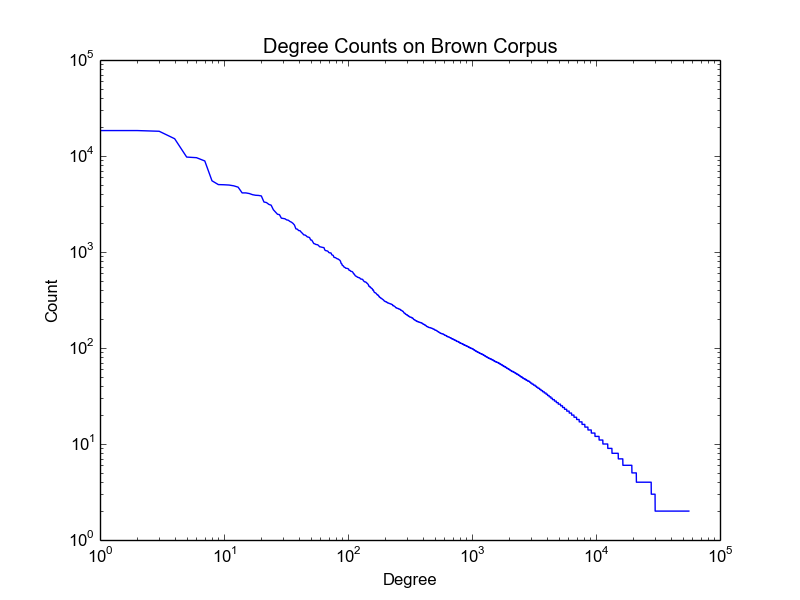
\includegraphics[width=0.19\textwidth]{degree_plot}
  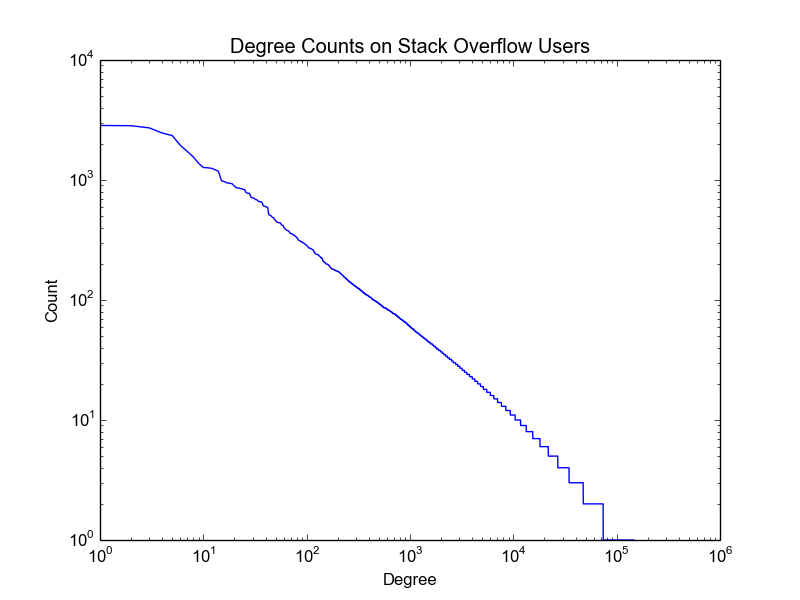
\includegraphics[width=0.19\textwidth]{overflow_degree_plot}
  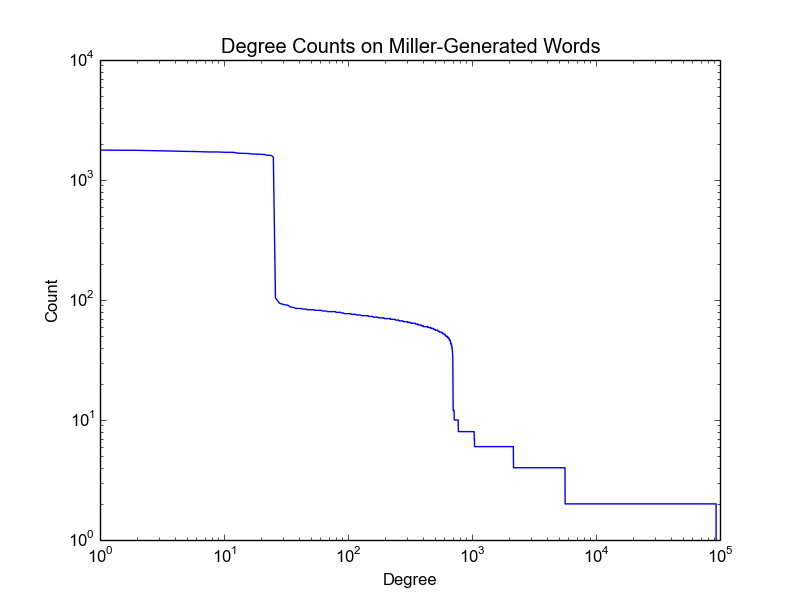
\includegraphics[width=0.19\textwidth]{miller_degree_plot}
  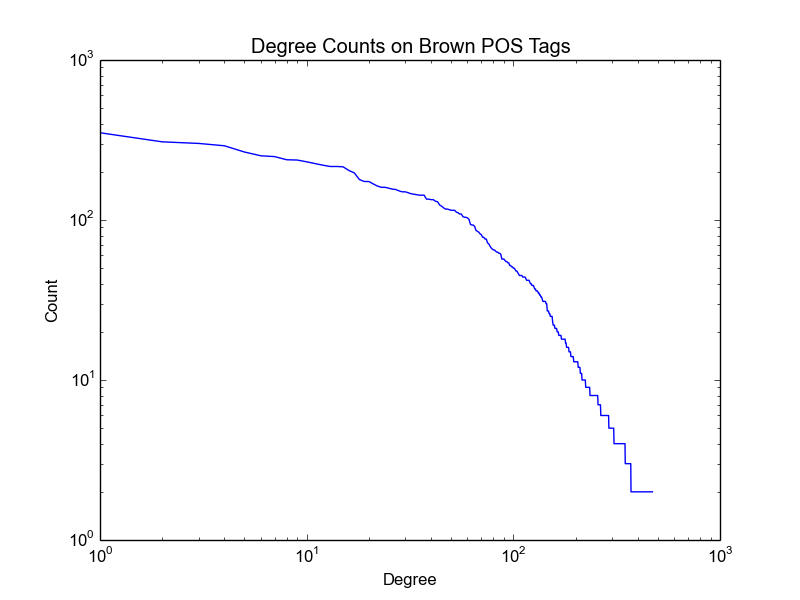
\includegraphics[width=0.19\textwidth]{pos_degree_plot}
  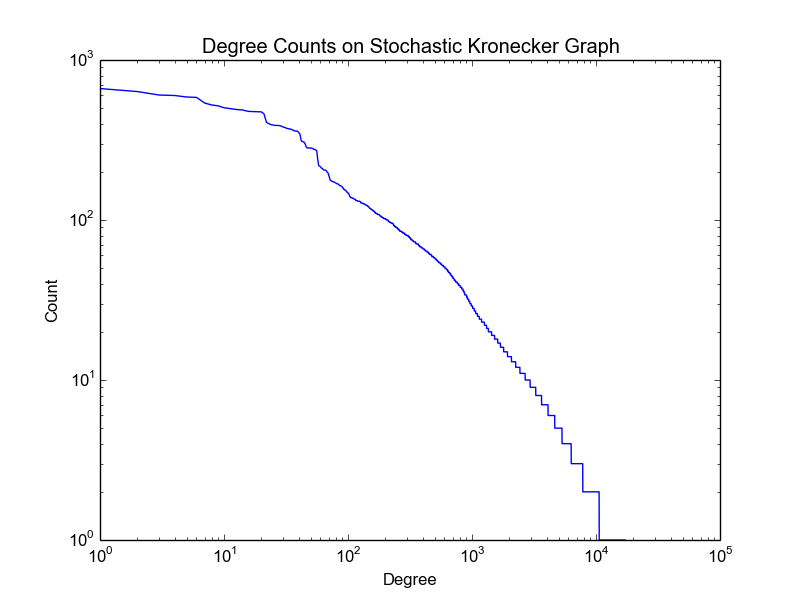
\includegraphics[width=0.19\textwidth]{kron_degree_plot}

  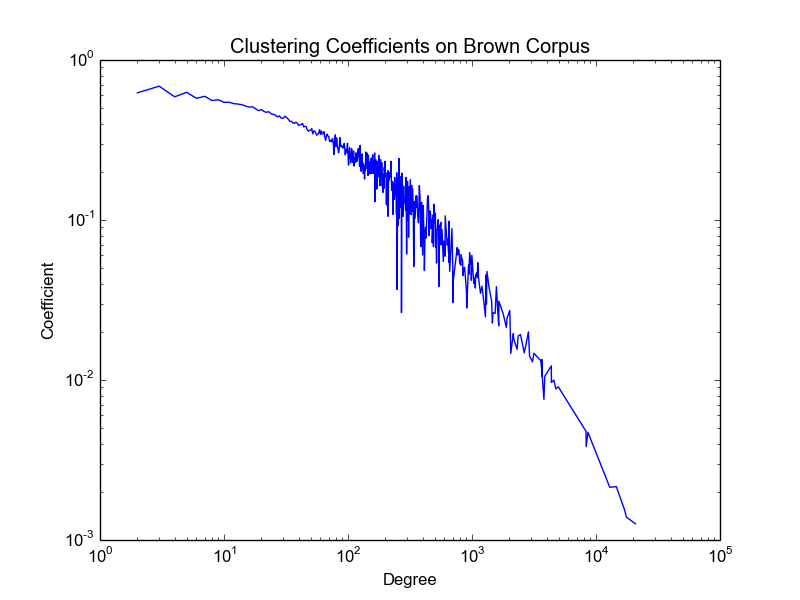
\includegraphics[width=0.19\textwidth]{clustering_coeff}
  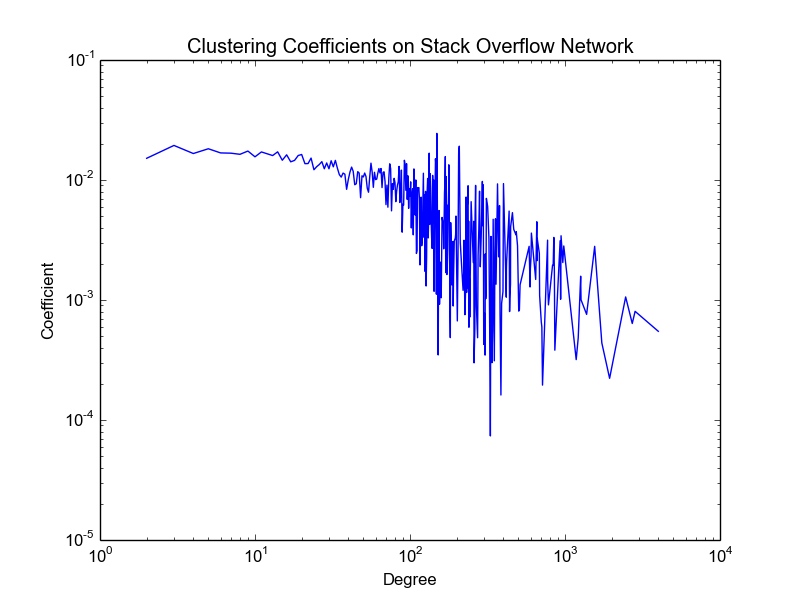
\includegraphics[width=0.19\textwidth]{overflow_clustering_coeff}
  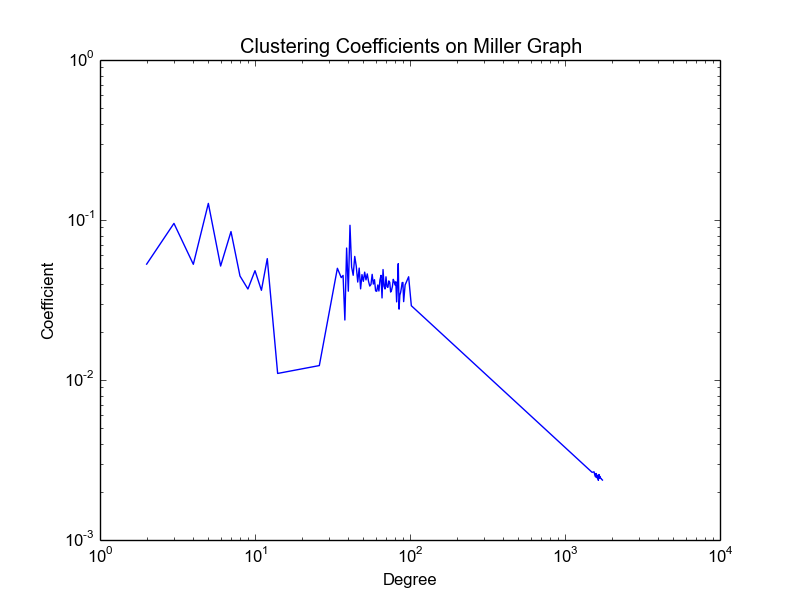
\includegraphics[width=0.19\textwidth]{miller_clustering_coeff}
  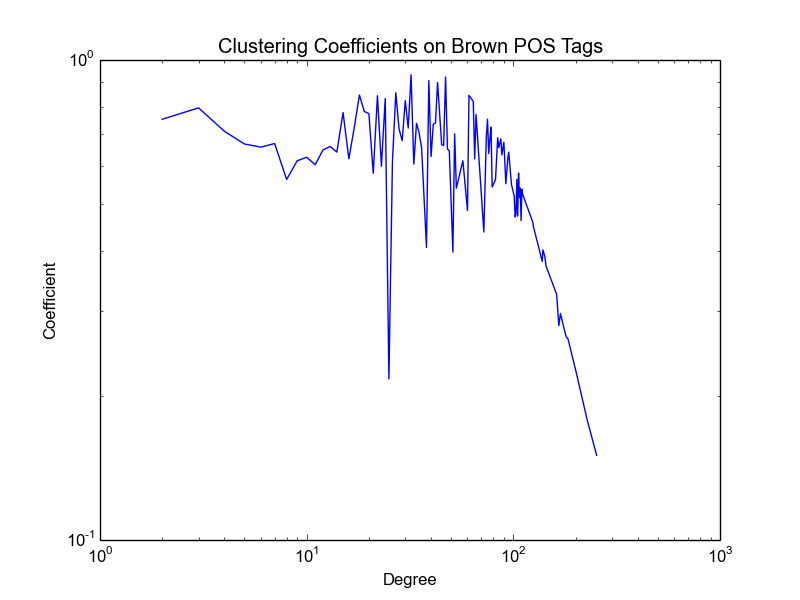
\includegraphics[width=0.19\textwidth]{pos_clustering_coeff}
  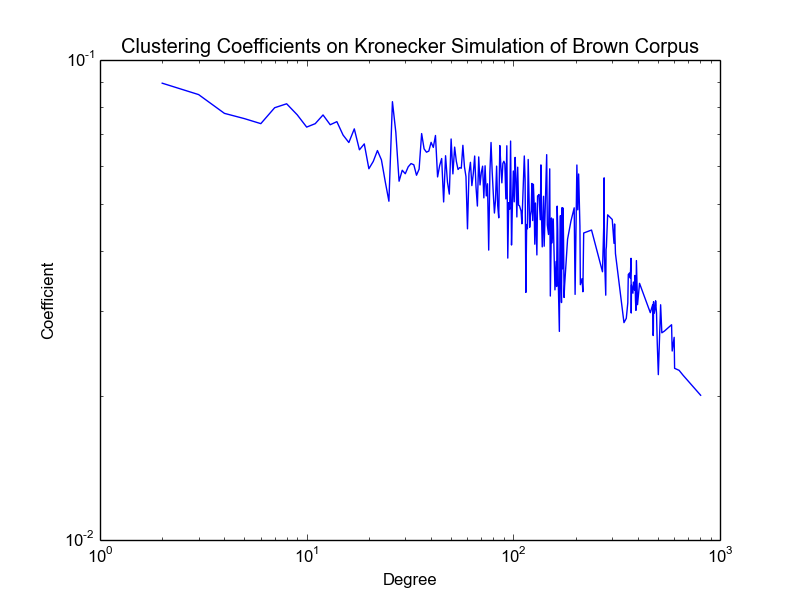
\includegraphics[width=0.19\textwidth]{kron_clustering_coeff}
  
  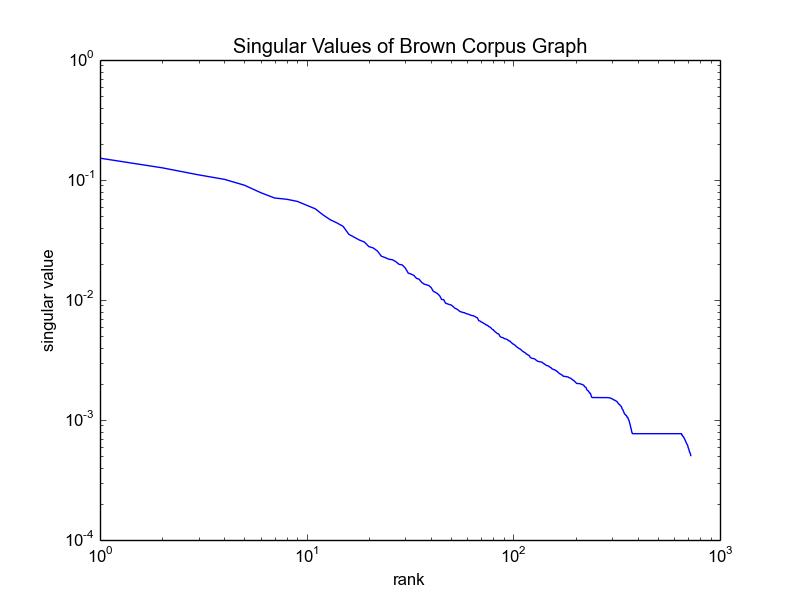
\includegraphics[width=0.19\textwidth]{singval_loglog}
  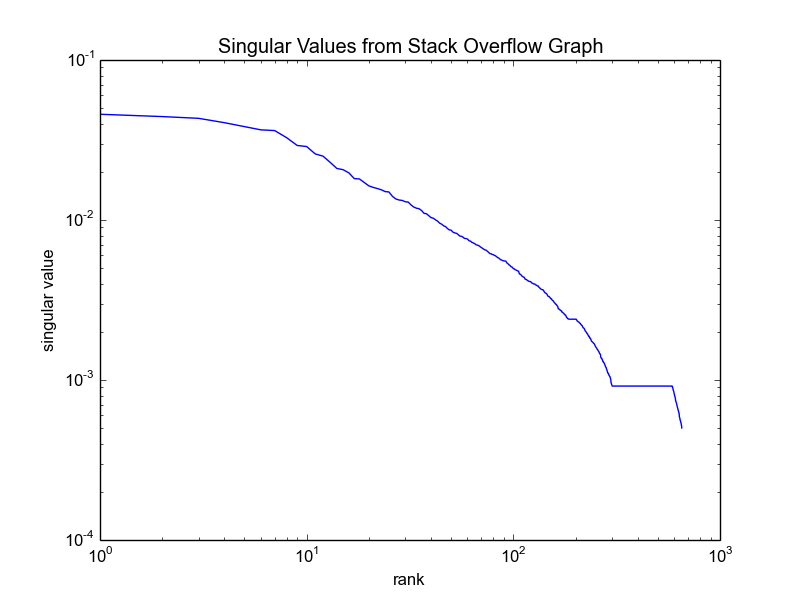
\includegraphics[width=0.19\textwidth]{overflow_singval_loglog}
  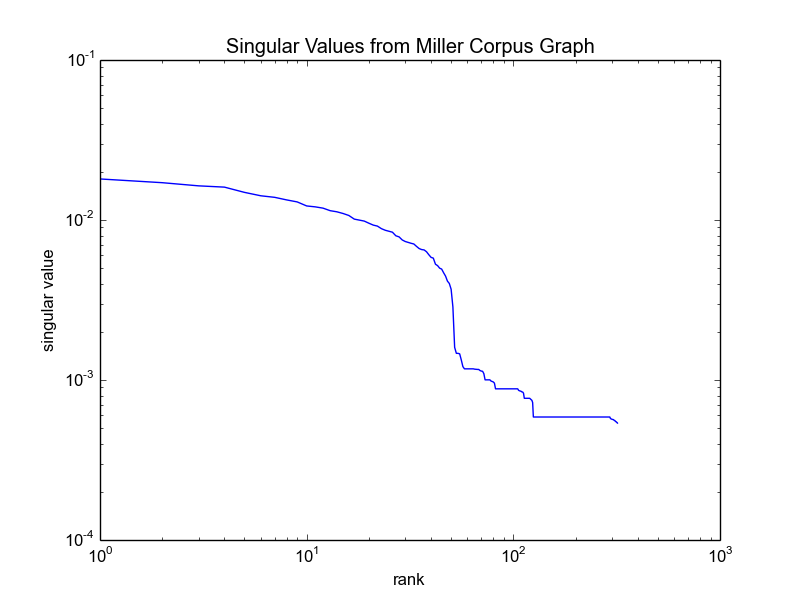
\includegraphics[width=0.19\textwidth]{miller_singval_loglog}
  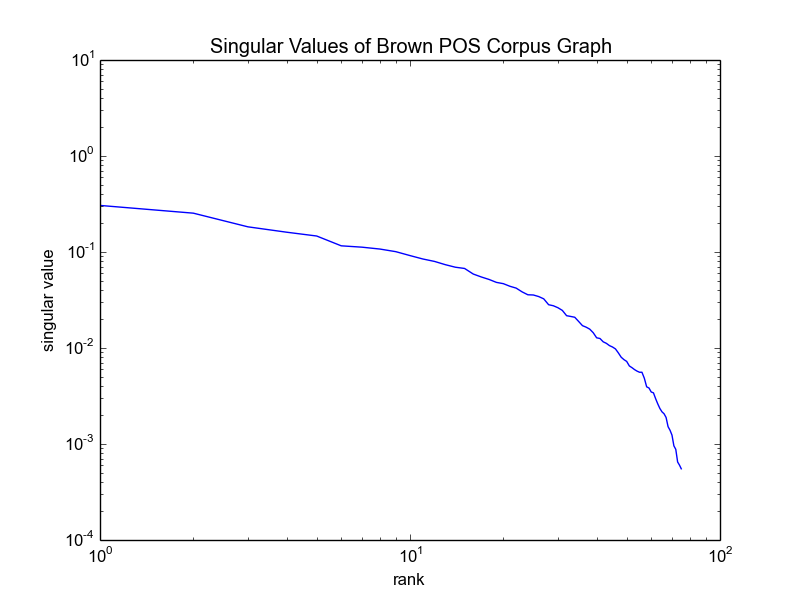
\includegraphics[width=0.19\textwidth]{pos_singval_loglog}
  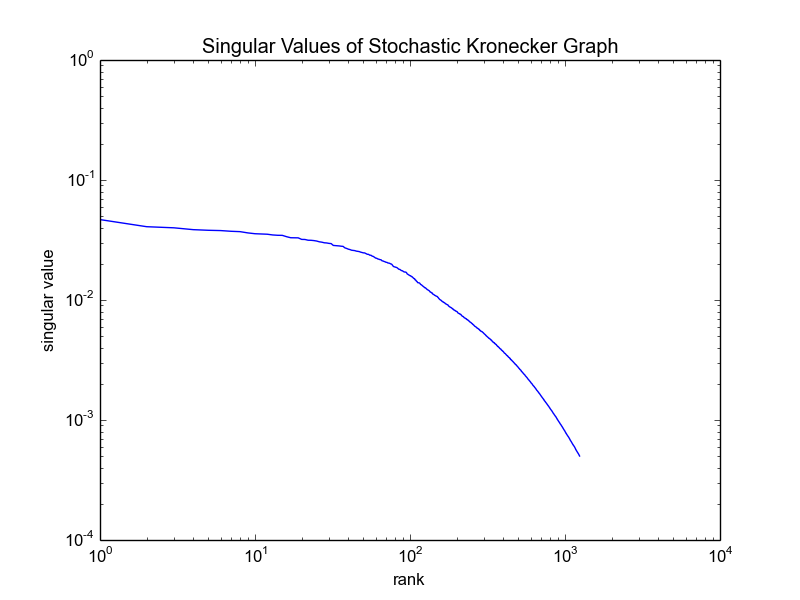
\includegraphics[width=0.19\textwidth]{kron_singval_loglog}
  
  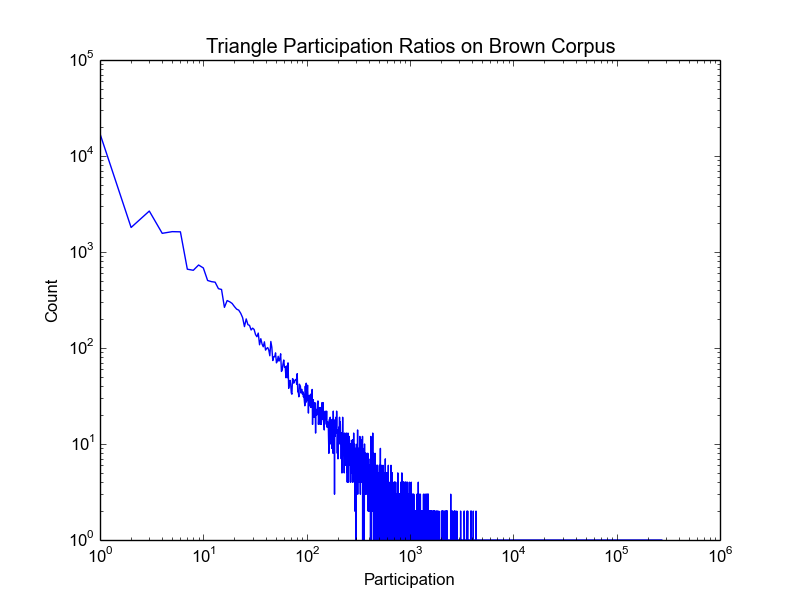
\includegraphics[width=0.19\textwidth]{triads}
  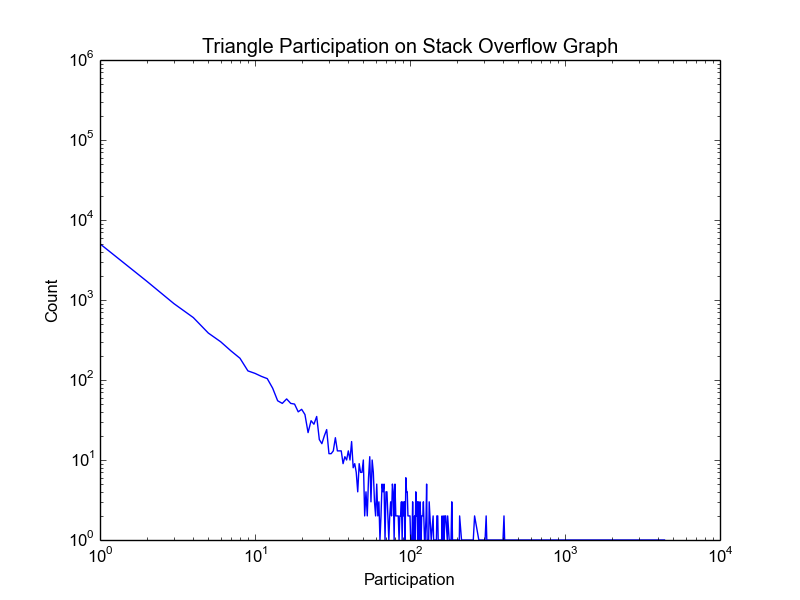
\includegraphics[width=0.19\textwidth]{overflow_triads}
  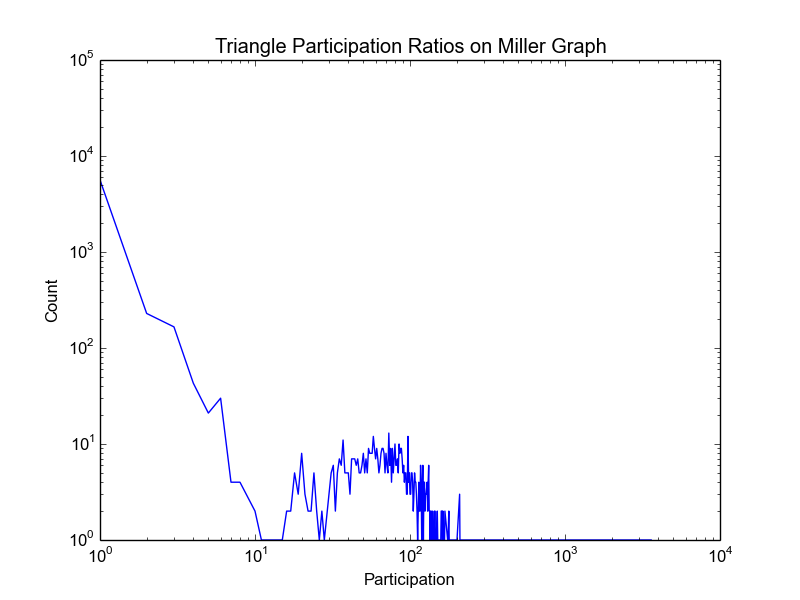
\includegraphics[width=0.19\textwidth]{miller_triads}
  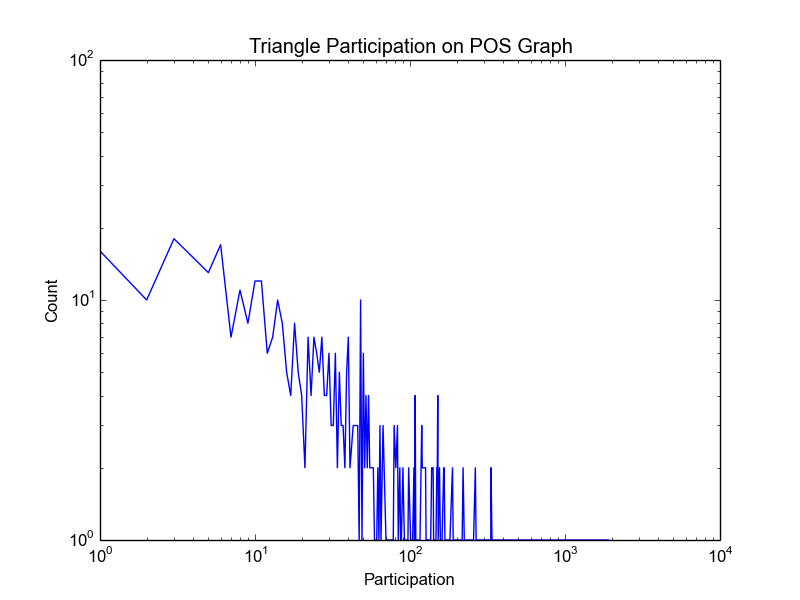
\includegraphics[width=0.19\textwidth]{pos_triads}
  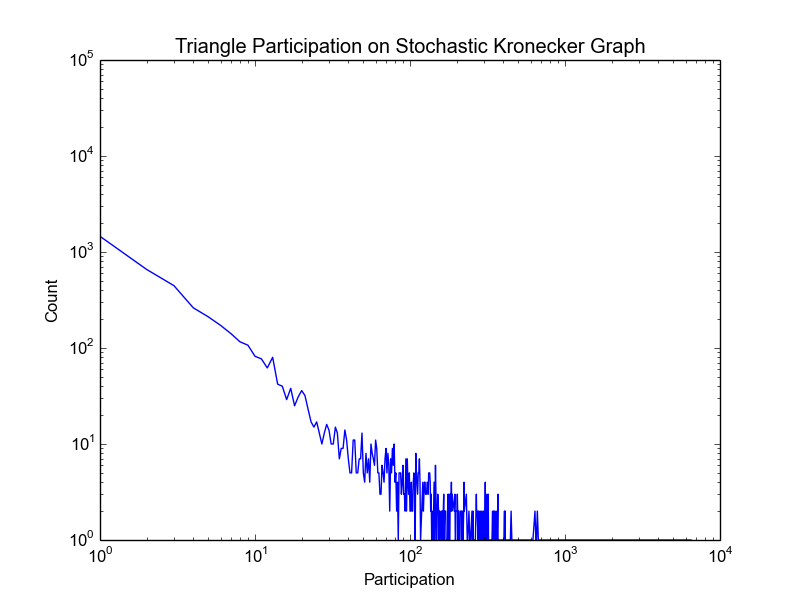
\includegraphics[width=0.19\textwidth]{kron_triads}

  \caption{Columns, left to right: Brown corpus graph, Stack Overflow questions graph, Miller graph, Brown POS tag graph, generated SKG graph (from Brown corpus fit). Rows, top to bottom: degree plot, clustering coefficients, singular values, triad participation}
\end{figure}

%%%% mturk: mturk people saying that the first one was good. conjecture that this scheme was all a bit bullshit.
%%%3. give an example of the damn generated text

\begin{figure}
  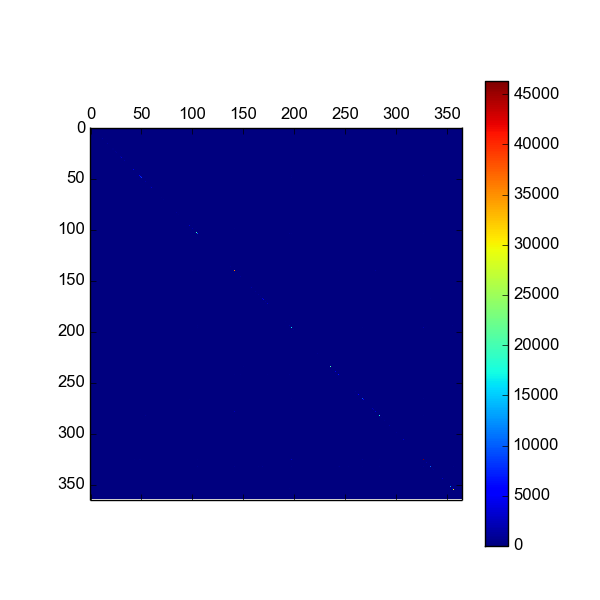
\includegraphics[width=0.19\textwidth]{kron_conf_mat}
  \caption{Confusion matrices for the parent feature tagger, to show imbalance of classes}
\end{figure}

%% 1. confusion matrix for the POS baseline and with all the Kronecker methods. Talk about how this is all bullshit, but for the trivial point that this is an imbalanced class. %%How many classes are there?

\begin{figure}
  \begin{tabular}{c || c | c | c | c | c}
    \hline
    . & Baseline & Bigram & Parents & Children & Degree \\
    \hline
    F1 & 0.289 & 0.332 & 0.299 & 0.261 & 0.288 \\
    Precision & 0.289 & 0.328 & 0.289 & 0.261 & 0.294 \\
    Recall & 0.328 & 0.366 & 0.341 & 0.279 & 0.315 \\
    Accuracy & 0.865 & 0.894 & 0.888 & 0.856 & 0.859 \\
    \hline
  \end{tabular}
  \caption{F1, precision, recall, accuracy for the respective taggers}
\end{figure}

%%% and a LOT of error analysis on the actual words themselves. talk about the idea that they have any actual grammar
%%% talk about the weights problem, note that it wasn't within the scope of the project really, it would probably explain the failure of the degrees

%we made the whole tagging system...

\begin{figure}
  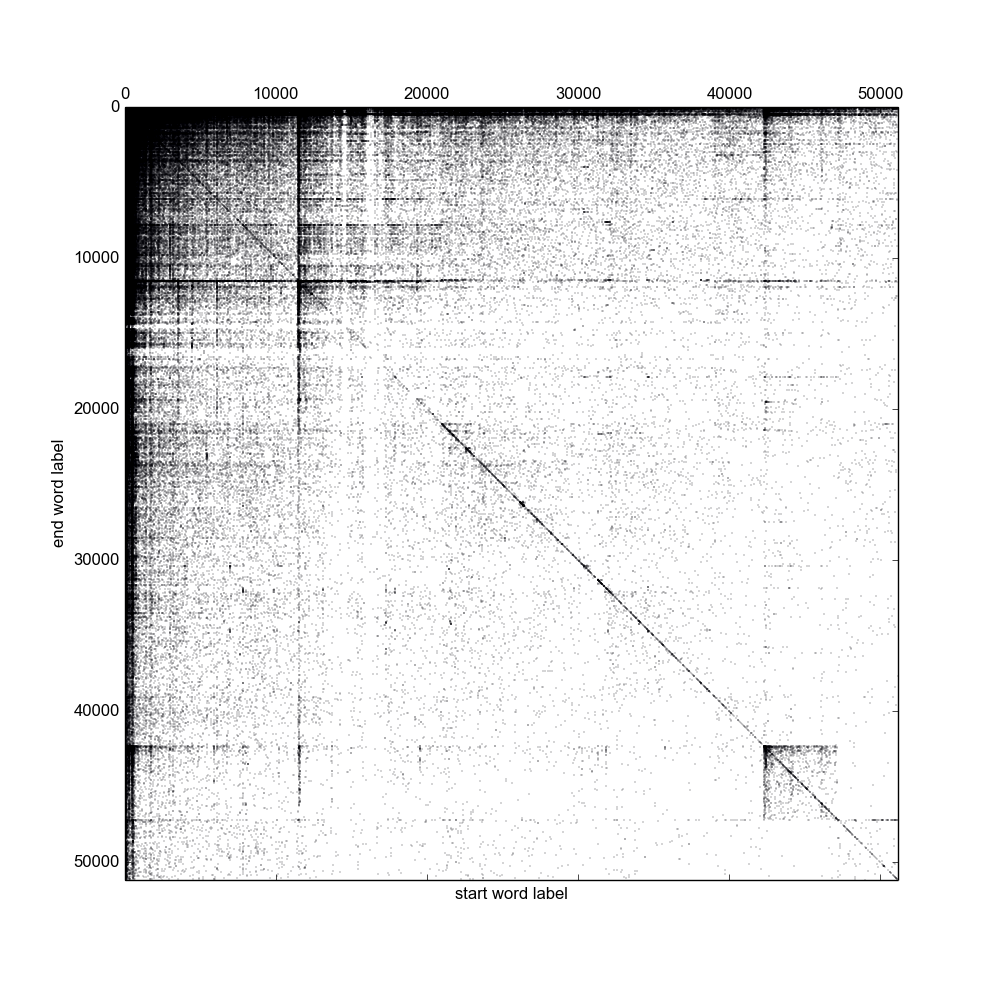
\includegraphics[width=0.45\textwidth]{bigram_sparsematplot.png}
  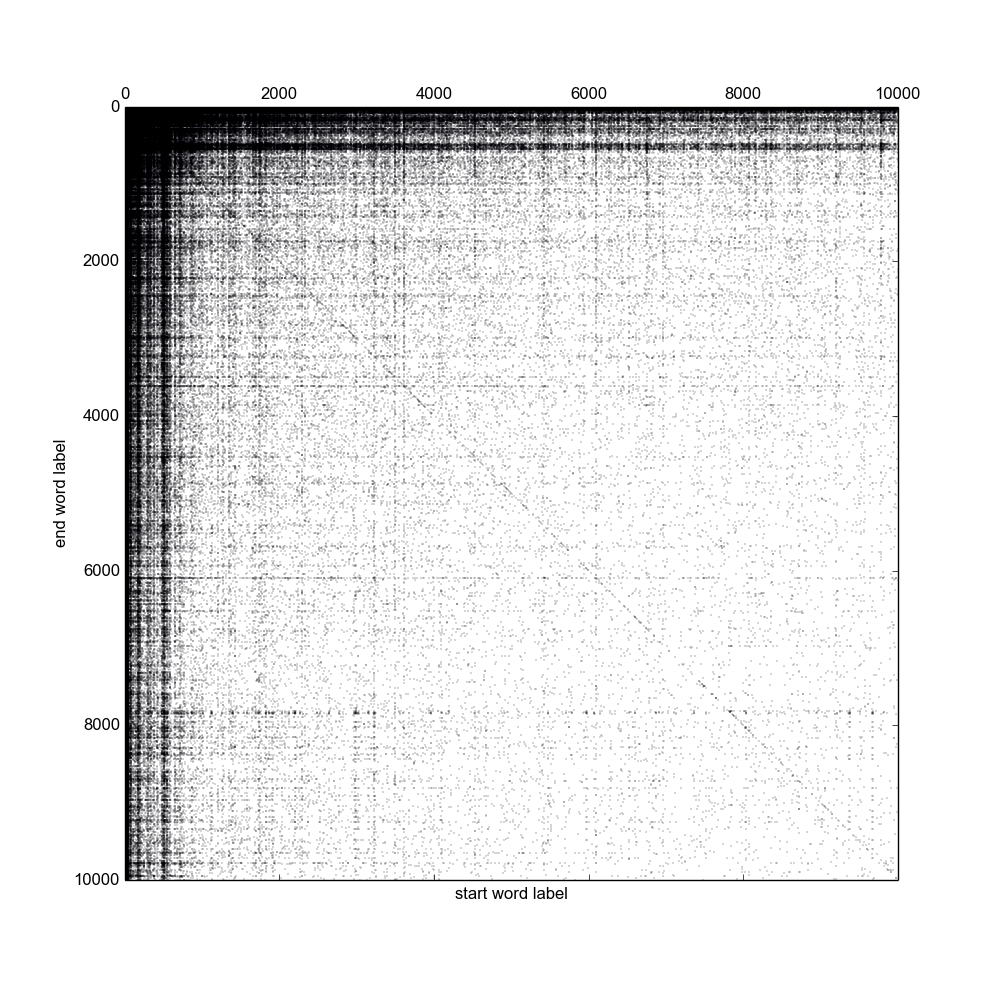
\includegraphics[width=0.45\textwidth]{bigram_small_sparsematplot.png}
  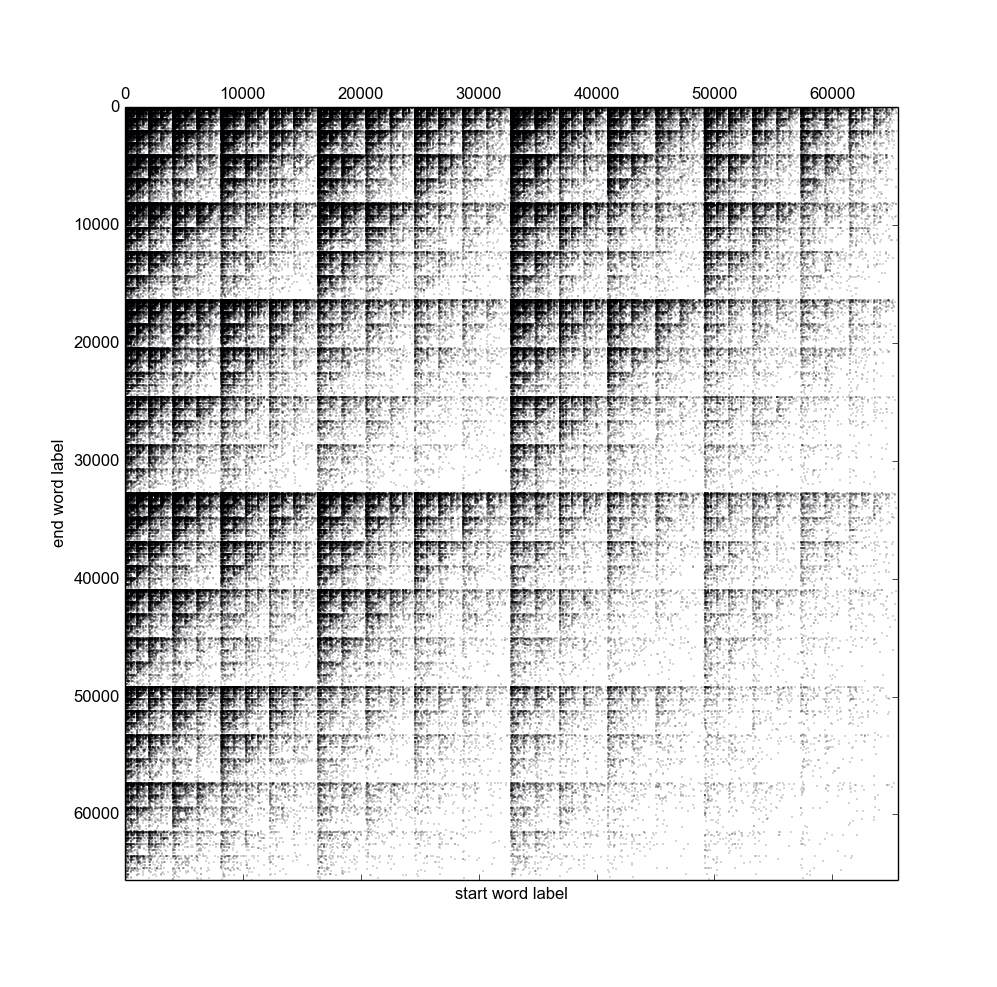
\includegraphics[width=0.45\textwidth]{kronfit2_sparsematplot.png}
  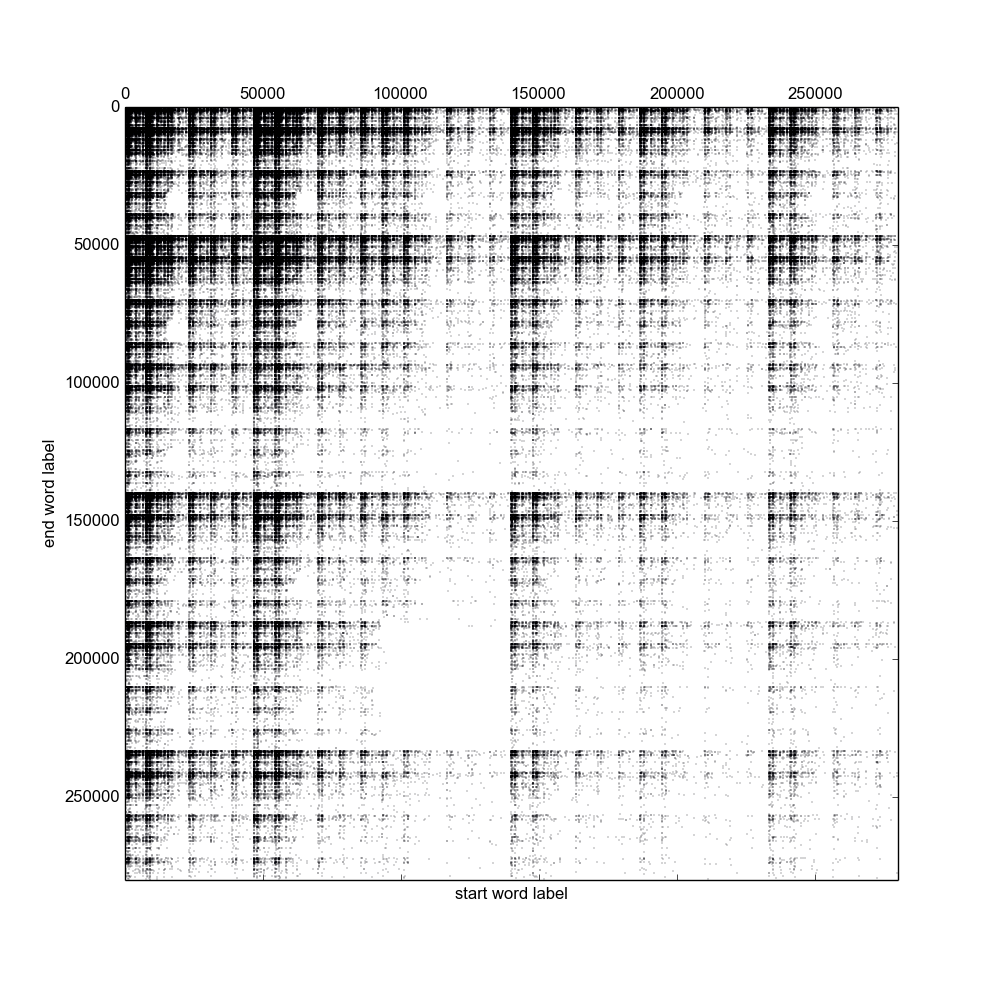
\includegraphics[width=0.45\textwidth]{kronfit6_sparsematplot.png}
  \caption{clockwise from top left: matrix plot(dots are edges) of bigram, matrix plot of $\frac{1}{5}$ of bigram, 6 by 6 Kronecker fit graph, 2 by 2 Kronecker fit graph}
\end{figure}

%%% convince the reader that Kronecker graphs would be good for this: it captures the degree structure, we can get good features from it
%%% convince the reader that Kronecker graphs have faults for this: talk about the weights. talk about the node matching problem. give an example of a mismatched node, maybe one with a fucked-up degree there

\subsection{Contributions}
There was only one person involved in the project. However, we have to note that much of the infrastructure of the Perceptron tagger was mutated from code by Matthew Honnibal of Macquarie University, and that we used SNAP and Networkx for the manipulation and analysis of language graphs. %cite that guy, snap, networkx, add MIT license back in again in the code. that's kosher, right?

%%% citations to add: snap, networkx, honiger, metzenmacher, RTG graph, some respected conll paper with averaged perceptron, the Brown corpus, Stack overflow corpus. add them in the text, too

\begin{thebibliography}{99}
  \bibitem{smallworldlang}
    Cancho, RF. and RV Sole. 2001. "The Small World of Human Language". Proceedings of the Royal Society B: Biological Sciences.
  \bibitem{kronfit}
    Lekovec, J., and Faloutsos, C. 2007. "Scalable Modeling of Real Graphs Using Kronecker Multiplication." Proceedings of ICML.
  \bibitem{mejpowerlaw}
    Newman, MEJ. 2005. "Power laws, Pareto distributions and Zipf's law." Contemporary Physics.
  \bibitem{fractaldim}
    Mandelbrot, BB., 1982. "The Fractal Geometry of Nature." WH Freeman and Company.
  \bibitem{lacunarity}
    Mandelbrot, BB., 1995. "Measures of Fractal Lacunarity: Minkowski Content and Alternatives". Fractal Geometry and Stochastics.
  \bibitem{richter}
    Stix, G. 1992. "Finding Fault." Scientific American.
  \bibitem{fractalcutoffs}
    Malcai, O., DA. Lidar, O. Biham and D. Avnir. 1998. "Scaling Range and Cutoffs in Empirical Fractals". Physical Review.
  \bibitem{netvalskew}
    Chakrabarti, D., Y. Zhan and C. Faloutsos. 2004. "R-mat: A recursive model for graph mining." SIAM Conference on Data Mining.
  \bibitem{densificationpowerlaw}
    Leskovec, J., JM Kleinberg and C. Faloutsos. 2007. "Graph evolution: Densification and shrinking diameters." ACM TKDD.
  \bibitem{stochkrongraph}
    Mahdian, M., and Y. Xu. 2007. "Stochastic Kronecker Graphs." Workshop on Algorithms and Models for the Web Graph.
  \bibitem{mlcompression}
    Frank, E., C. Chui and IH. Witten. 2000. "Text Categorization using Compression Models." IEEE Data Compression.
  \bibitem{cosma}
    Clauset, A., CR Shalizi and MEJ Newman. 2009. "Power-law distributions in empirical data." SIAM Review.
  \bibitem{gamiller}
    Miller, GA. 1957. "Some Effects of Intermittent Silence". The American Journal of Psychology.
  \bibitem{shannon}
    Shannon, C. E., 1950. "Prediction and Entropy of Printed English". Bell System Technical Journal.
  \bibitem{nltk}
    Bird, Steven, Edward Loper and Ewan Klein, 2009. "Natural Language Processing with Python." O'Reilly Media Inc.
  \bibitem{collins}
    Collins, Michael. 2011. "Tagging with Hidden Markov Models".
\end{thebibliography}


\end{document}
